\chapter{Tests}

In diesem Kapitel wird das Konzept des Tests beschrieben, da die Korrektheit der Erweiterung anhand von Tests verifiziert werden soll.
Die damit verbundenen Parameter und Abläufe werden in den nächsten Seiten festgehalten.


\section{Der Test-Plan}

Um zu verifizieren, dass die in dieser Masterarbeit entwickelte BCI-Erweiterung funktioniert, muss diese getestet werden.
Nachfolgend werden die einzelnen Bestandteile des Tests aufgeführt, die im Laufe dieses Kapitels genauer definiert 
und in einen sinnvollen Zusammenhang gebracht werden.

\begin{itemize}
\item Einführung zum Testablaufs und Einverständniserklärung
\item Fragebögen zur Ermittlung relevanter Informationen
\item Kalibrierung des BCI mittels P300-Speller
\item Vorher-Test der Kalibrierung
\item Durchführung des Test-Spiels mit dem AGS-P300-Speller
\item Nachher-Test der Kalibrierung
\item Ermittlung der subjektiven Belastung\\
\end{itemize}


\subsubsection{Ablauf des Tests}

Zu Beginn wird jeder Testperson der Ablauf des Tests erklärt.
Sollte eine Person allergisch auf Kontaktlinsenflüssigkeit sein, dann wäre der Test an dieser Stelle beendet, da diese zum Befeuchten der Elektroden verwendet wird.
Ansonsten wird jeder Proband gebeten eine Einverständniserklärung für die anonyme Verwendung der Daten innerhalb dieser Arbeit zu unterzeichnen.\\

Sobald der Test beginnen kann, muss zunächst ein Fragebogen ausgefüllt werden.
Dieser sammelt relevante Daten zur Einordnung der Testpersonen.
Anschließend beginnt die Kalibrierung des Emotiv EPOC mit Hilfe des P300-Spellers.
Sobald das BCI kalibriert ist werden der "`Vorher-Test"', das Test-Spiel und der "`Nacher-Test"' durchgeführt.
Vor der Kalibrierung und dem Test-Spiel, sowie vor und nach dem "`Nachher-Test"' wird jeweils ein kurzer Fragebogen ausgefüllt, der das Befinden der Testpersonen festhält.
Dies ist der Tatsache geschuldet, dass eine Verschlechterung der Ergebnisse auf Ermüdung durch die ungewohnte Belastung zurückgeführt werden könnte.
Nach dem Ausfüllen des letzten Fragebogens ist der Test abgeschlossen.
Alle verwendeten Fragebögen finden sich im Anhang ab Seite \pageref{anhang}.\\



\subsubsection{Kalibrierung des \acs{BCI}'s}

Bevor die einzelnen Speller-Tests beginnen können, muss das \acs{BCI} kalibriert werden.
Zu diesem Zweck muss jeder Probant zunächst die beiden Wörter \mbox{"`BRAIN"'} und \mbox{"`ISLAND"'} mit dem P300-Speller schreiben.
Die für die Kalibrierung und die Tests erforderlichen Testparameter wurden zuvor durch einzelne Tests mit einer geübten und einer ungeübten Testperson ermittelt.
Die daraus hervorgehenden Parameter wurden insbesondere in Bezug auf ungeübte Personen ausgewählt, 
da die Mehrheit der Testpersonen erwartungsgemäß keine Erfahrung im Umgang mit \acs{BCI}s vorweisen können.
\begin{itemize}
\item PreSequenceDuration: 2000ms
\item PostSequenceDuration: 2000ms
\item StimulusDuration: 125ms
\item InterStimulusDuration: 125-250ms
\item NumberOfSequences: 10 \\
\end{itemize}
Diese Parameter bestimmen die Wartezeit vor und nach jeder Stimuli-Sequenz, der Zeit \mbox{einer} Stimuli-Visualisierung und der Zeit zwischen zwei Stimuli-Visualisierungen.
Die Wartezeit zwischen den Sequenzen ist bewusst auf einem etwas höheren Wert festgelegt, da die Testpersonen den neuen Buchstaben vor der nächsten Sequenz finden und fokussieren müssen.
Die Dauer einer Sequenz beträgt das zehnfache der einfachen Sequenz, so dass jede Zeile bzw. Spalte zehn mal hervorgehoben wird.
Anhand der dadurch ermittelten Daten wird eine Klassifizierung mit dem "`P300-Classifier"' des BCI2000-Frameworks durchgeführt, 
die Klassifizierung führt hierfür eine \ac{SWLDA} durch \cite[S.208ff]{schalk2010practical}.
Dieser generiert Parameter die vom Speller geladen werden müssen, um individuelle Unterschiede der Probanden zu berücksichtigen.
Im Anschluss daran wird der Referenz-Test 1 durchgeführt.




\subsubsection{Referenz-Test 1 \& 2}
Bei der Verwendung von \acs{BCI}'s kann die Qualität der Ergebnisse je nach Individuum stark variieren.
Aus diesem Grund werden die Parameter der Klassifizierung im Referenz-Test 1 angewendet, um Aussagen über die relative Genauigkeit zu erhalten.
Um die Ergebnisse des Test-Spiels einordnen zu können wird ein zusätzlicher Referenz-Test 2 nach dem Test-Spiel durchgeführt.
Dieser ist vom Aufbau her äquivalent zum Referenz-Test 1.
Beide Tests dienen als Vergleichsreferenz für das Test-Spiel.\\

Um zu zeigen, dass die BCI-Erweiterung korrekt funktioniert, müssen die Ergebnisse des Test-Spiels eine ähnliche Genauigkeit wie Referenz-Test 1 besitzen.
Sollten die Ergebnisse hingegen schlechter sein, muss Referenz-Test 2 zum Vergleich hinzugezogen werden.
Auf diese Weise kann eine mögliche Ermüdung des Nutzers gezeigt oder ausgeschlossen werden.\\



\subsubsection{Durchführung des Test-Spiels}

Während des Test-Spiels müssen die Probanden mit der Spielfigur alle Objekte im Spiel aufheben, die Szene nach rechts wechseln und alle dort verbliebenen Objekte aufheben.
Jedes richtig ausgewählte Matrix-Element ist ein Treffer, jedes falsch ausgewählte ein Fehler. 
Die Befehle werden jeweils in einer Spalte durch fünf verschiedene Matrix-Elemente repräsentiert, daher haben die Probanden die Anweisung immer das mittlere Element auszuwählen, 
weil dieses den Schriftzug des Befehls enthält.
Die korrekte Spalte bei falscher Zeile würde den richtigen Befehl auswählen, jedoch trotzdem als Fehler bewertet werden.
In Abbildung \ref{befehlsmatrix} ist dies beispielhaft für die Auswahl des Befehls "`Aufheben"' dargestellt.\\

\pagebreak

\begin{figure}[h!]
\begin{center}
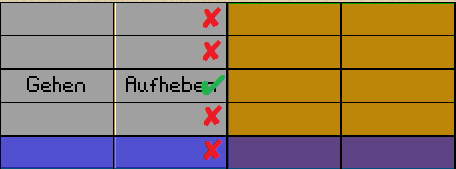
\includegraphics[scale=0.65]{images/BefehlsauswahlHitMiss.png}
\caption{Ein Ausschnitt der Speller-Matrix der Befehlsleiste. Die fünf Felder der Spalte \textit{Aufheben} wählen alle den selben Befehl aus, jedoch wird nur das Feld mit dem grünen Hakens als Treffer gewertet.}
\label{befehlsmatrix}
\end{center}
\end{figure}


Das Spiel wird beendet, sobald alle Objekte aufgehoben sind oder 25 Eingabe-Ermittlungen erreicht sind.
Die relative Genauigkeit jeder Testperson wird am Ende anhand der Treffer und Fehler ermittelt.
Das Ergebnis kann im Anschluss mit den Referenz-Tests verglichen und bewertet werden.\\



\subsubsection{Der NASA Task Load Index}
Im Anschluss an den gesamten Test muss jede der Testpersonen einen weiteren Fragebogen ausfüllen.
Dieser sogenannte \ac{NASA-TLX} \cite{hart1988development} umfasst sechs multidimensionale Bewertungen anhand derer eine subjektive Gesamtbelastung errechnet wird.
Die Bewertungen sind nachfolgend aufgeführt.

\begin{itemize}
\item Geistige Anforderungen
\item Körperliche Anforderungen
\item Zeitliche Anforderungen
\item Aufgabenerfüllung
\item Anstrengung
\item Frustration \\
\end{itemize}

Die ersten drei Punkte beziehen sich in erster Linie auf die Testperson, während die letzten drei Punkte die Durchführung der Aufgabe einbeziehen.
Die Erläuterungen der einzelnen Bewertungskriterien sind in Tabelle \ref{table:nasatlx} kurz dargestellt.

\begin{center}
\begin{table}[h!]
    \begin{tabular}{ | l | l | p{6cm} |}
    \hline
	\rule{0pt}{4ex} 
	\textbf{Bewertung} & \textbf{Skala} & \textbf{Erläuterung} \\ \hline 
	\rule{0pt}{4ex} 
    Geistige Anforderungen & gering/hoch & Wie gering/hoch war die geistige Beanspruchung? \\ \hline 
	\rule{0pt}{4ex} 
    Körperliche Anforderungen & gering/hoch & Wie gering/hoch war die körperliche Belastung?  \\ \hline
	\rule{0pt}{4ex} 
    Zeitliche Anforderungen & gering/hoch & Wie hoch war der zeitliche Druck? \\ \hline
	\rule{0pt}{4ex} 
    Aufgabenerfüllung & gut/schlecht & Wie gut empfand die Testperson ihr Ergebnis? \\ \hline
	\rule{0pt}{4ex} 
	Anstrengung & gering/hoch & Wie anstrengend war die Aufgabe für die Testperson? \\ \hline
	\rule{0pt}{4ex} 
	Frustration & gering/hoch & Wie frustierend war die Aufgabe für die Testperson? \\ \hline

	\end{tabular}
\caption{Die Bewertungskriterien des \acs{NASA-TLX}}
\label{table:nasatlx}
\end{table}
\end{center}

\pagebreak
Um die subjektive Gesamtbelastung zu berechnen wird zunächst die Gewichtung der Beanspruchungsstruktur ermittelt.
Dabei werden die einzelnen Bewertungskriterien gegenübergestellt, sodass die Testperson das jeweils ihrer Meinung nach wichtigere auswählt.
Im nächsten Schritt muss jedes Kriteriums anhand der Skala in Tabelle \ref{table:nasatlx} eingeordnet werden, um eine Wertung ablesen zu können.
Die Wertungen und Gewichtungen werden miteinander verrechnet, sodass sich eine durschnittliche Gesamtbelastung ergibt.
Die deutsche Fassung der \acs{NASA-TLX}-Fragebögen \cite{seifert02} befinden sich im Anhang dieser Arbeit.\\





%   Da die Aufzeichnung der \acs{P300 ERP}'s mittels des von der Universität bereitgestellten Emotiv EPOC durchgeführt werden.
%   P3,P4,PO8,Fz,Cz,Pz,PO7,Oz http://www.bci2000.org/phpbb/viewtopic.php?t=390




